\documentclass[twoside]{book}

% Packages required by doxygen
\usepackage{calc}
\usepackage{doxygen}
\usepackage{graphicx}
\usepackage[utf8]{inputenc}
\usepackage{makeidx}
\usepackage{multicol}
\usepackage{multirow}
\usepackage{textcomp}
\usepackage[table]{xcolor}

% Font selection
\usepackage[T1]{fontenc}
\usepackage{mathptmx}
\usepackage[scaled=.90]{helvet}
\usepackage{courier}
\usepackage{amssymb}
\usepackage{sectsty}
\renewcommand{\familydefault}{\sfdefault}
\allsectionsfont{%
  \fontseries{bc}\selectfont%
  \color{darkgray}%
}
\renewcommand{\DoxyLabelFont}{%
  \fontseries{bc}\selectfont%
  \color{darkgray}%
}

% Page & text layout
\usepackage{geometry}
\geometry{%
  a4paper,%
  top=2.5cm,%
  bottom=2.5cm,%
  left=2.5cm,%
  right=2.5cm%
}
\tolerance=750
\hfuzz=15pt
\hbadness=750
\setlength{\emergencystretch}{15pt}
\setlength{\parindent}{0cm}
\setlength{\parskip}{0.2cm}
\makeatletter
\renewcommand{\paragraph}{%
  \@startsection{paragraph}{4}{0ex}{-1.0ex}{1.0ex}{%
    \normalfont\normalsize\bfseries\SS@parafont%
  }%
}
\renewcommand{\subparagraph}{%
  \@startsection{subparagraph}{5}{0ex}{-1.0ex}{1.0ex}{%
    \normalfont\normalsize\bfseries\SS@subparafont%
  }%
}
\makeatother

% Headers & footers
\usepackage{fancyhdr}
\pagestyle{fancyplain}
\fancyhead[LE]{\fancyplain{}{\bfseries\thepage}}
\fancyhead[CE]{\fancyplain{}{}}
\fancyhead[RE]{\fancyplain{}{\bfseries\leftmark}}
\fancyhead[LO]{\fancyplain{}{\bfseries\rightmark}}
\fancyhead[CO]{\fancyplain{}{}}
\fancyhead[RO]{\fancyplain{}{\bfseries\thepage}}
\fancyfoot[LE]{\fancyplain{}{}}
\fancyfoot[CE]{\fancyplain{}{}}
\fancyfoot[RE]{\fancyplain{}{\bfseries\scriptsize Generated on Mon Nov 16 2015 21\-:52\-:57 for My Project by Doxygen }}
\fancyfoot[LO]{\fancyplain{}{\bfseries\scriptsize Generated on Mon Nov 16 2015 21\-:52\-:57 for My Project by Doxygen }}
\fancyfoot[CO]{\fancyplain{}{}}
\fancyfoot[RO]{\fancyplain{}{}}
\renewcommand{\footrulewidth}{0.4pt}
\renewcommand{\chaptermark}[1]{%
  \markboth{#1}{}%
}
\renewcommand{\sectionmark}[1]{%
  \markright{\thesection\ #1}%
}

% Indices & bibliography
\usepackage{natbib}
\usepackage[titles]{tocloft}
\setcounter{tocdepth}{3}
\setcounter{secnumdepth}{5}
\makeindex

% Hyperlinks (required, but should be loaded last)
\usepackage{ifpdf}
\ifpdf
  \usepackage[pdftex,pagebackref=true]{hyperref}
\else
  \usepackage[ps2pdf,pagebackref=true]{hyperref}
\fi
\hypersetup{%
  colorlinks=true,%
  linkcolor=blue,%
  citecolor=blue,%
  unicode%
}

% Custom commands
\newcommand{\clearemptydoublepage}{%
  \newpage{\pagestyle{empty}\cleardoublepage}%
}


%===== C O N T E N T S =====

\begin{document}

% Titlepage & ToC
\hypersetup{pageanchor=false}
\pagenumbering{roman}
\begin{titlepage}
\vspace*{7cm}
\begin{center}%
{\Large My Project }\\
\vspace*{1cm}
{\large Generated by Doxygen 1.8.6}\\
\vspace*{0.5cm}
{\small Mon Nov 16 2015 21:52:57}\\
\end{center}
\end{titlepage}
\clearemptydoublepage
\tableofcontents
\clearemptydoublepage
\pagenumbering{arabic}
\hypersetup{pageanchor=true}

%--- Begin generated contents ---
\chapter{R\-E\-A\-D\-M\-E}
\label{md_README}
\hypertarget{md_README}{}
S\-E\-N\-G 330, Assignment 2 
\chapter{Hierarchical Index}
\section{Class Hierarchy}
This inheritance list is sorted roughly, but not completely, alphabetically\-:\begin{DoxyCompactList}
\item \contentsline{section}{machine}{\pageref{classmachine}}{}
\begin{DoxyCompactList}
\item \contentsline{section}{bracelet}{\pageref{classbracelet}}{}
\item \contentsline{section}{elliptical}{\pageref{classelliptical}}{}
\item \contentsline{section}{lift}{\pageref{classlift}}{}
\end{DoxyCompactList}
\item \contentsline{section}{member}{\pageref{classmember}}{}
\begin{DoxyCompactList}
\item \contentsline{section}{bracelet}{\pageref{classbracelet}}{}
\end{DoxyCompactList}
\item Message\begin{DoxyCompactList}
\item \contentsline{section}{machines\-:\-:Machine}{\pageref{classmachines_1_1Machine}}{}
\item \contentsline{section}{machines\-:\-:Machines}{\pageref{classmachines_1_1Machines}}{}
\end{DoxyCompactList}
\item \contentsline{section}{machines\-:\-:Static\-Descriptor\-Initializer\-\_\-fitplanet\-\_\-2eproto}{\pageref{structmachines_1_1StaticDescriptorInitializer__fitplanet__2eproto}}{}
\end{DoxyCompactList}

\chapter{Class Index}
\section{Class List}
Here are the classes, structs, unions and interfaces with brief descriptions\-:\begin{DoxyCompactList}
\item\contentsline{section}{\hyperlink{classbracelet}{bracelet} }{\pageref{classbracelet}}{}
\item\contentsline{section}{\hyperlink{classelliptical}{elliptical} }{\pageref{classelliptical}}{}
\item\contentsline{section}{\hyperlink{classlift}{lift} }{\pageref{classlift}}{}
\item\contentsline{section}{\hyperlink{classmachines_1_1Machine}{machines\-::\-Machine} }{\pageref{classmachines_1_1Machine}}{}
\item\contentsline{section}{\hyperlink{classmachine}{machine} }{\pageref{classmachine}}{}
\item\contentsline{section}{\hyperlink{classmachines_1_1Machines}{machines\-::\-Machines} }{\pageref{classmachines_1_1Machines}}{}
\item\contentsline{section}{\hyperlink{classmember}{member} }{\pageref{classmember}}{}
\item\contentsline{section}{\hyperlink{structmachines_1_1StaticDescriptorInitializer__fitplanet__2eproto}{machines\-::\-Static\-Descriptor\-Initializer\-\_\-fitplanet\-\_\-2eproto} }{\pageref{structmachines_1_1StaticDescriptorInitializer__fitplanet__2eproto}}{}
\end{DoxyCompactList}

\chapter{Class Documentation}
\hypertarget{classbracelet}{\section{bracelet Class Reference}
\label{classbracelet}\index{bracelet@{bracelet}}
}
Inheritance diagram for bracelet\-:\begin{figure}[H]
\begin{center}
\leavevmode
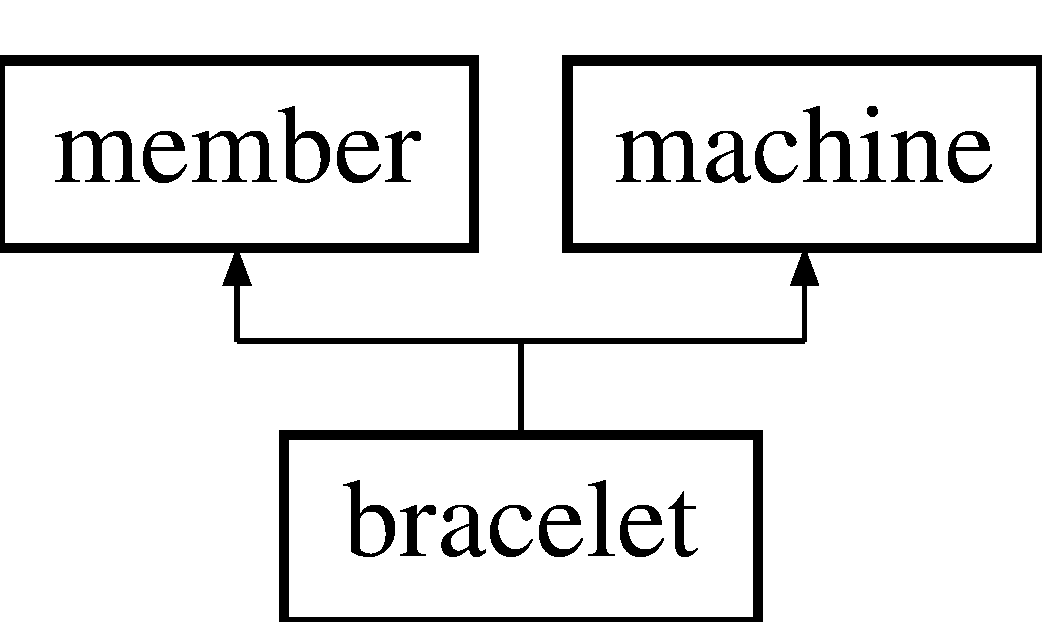
\includegraphics[height=2.000000cm]{classbracelet}
\end{center}
\end{figure}
\subsection*{Public Member Functions}
\begin{DoxyCompactItemize}
\item 
\hypertarget{classbracelet_a51b4e2907d3bd742bed3c5af8fb58e41}{{\bfseries bracelet} (char $\ast$)}\label{classbracelet_a51b4e2907d3bd742bed3c5af8fb58e41}

\item 
\hypertarget{classbracelet_a220850e5494aea041478ba50540ea58f}{char $\ast$ {\bfseries get\-\_\-owner} () const }\label{classbracelet_a220850e5494aea041478ba50540ea58f}

\item 
\hypertarget{classbracelet_a5df367d5e2c766f8070d892ed0735858}{std\-::vector$<$ \hyperlink{classmachine}{machine} $>$ {\bfseries machines\-\_\-used} () const }\label{classbracelet_a5df367d5e2c766f8070d892ed0735858}

\item 
\hypertarget{classbracelet_a7b27c0f1916a5a2ca1036e2f966ad431}{void {\bfseries change\-\_\-owner} (char $\ast$)}\label{classbracelet_a7b27c0f1916a5a2ca1036e2f966ad431}

\item 
\hypertarget{classbracelet_af335417478ad987d9df5521c430ac59d}{void {\bfseries remove\-\_\-owner} ()}\label{classbracelet_af335417478ad987d9df5521c430ac59d}

\item 
\hypertarget{classbracelet_a39485b59c215f4952da18b3bdb5aede0}{void {\bfseries add\-\_\-machine} (\hyperlink{classmachine}{machine})}\label{classbracelet_a39485b59c215f4952da18b3bdb5aede0}

\end{DoxyCompactItemize}


The documentation for this class was generated from the following files\-:\begin{DoxyCompactItemize}
\item 
bracelet.\-h\item 
bracelet.\-cpp\end{DoxyCompactItemize}

\hypertarget{classelliptical}{\section{elliptical Class Reference}
\label{classelliptical}\index{elliptical@{elliptical}}
}
Inheritance diagram for elliptical\-:\begin{figure}[H]
\begin{center}
\leavevmode
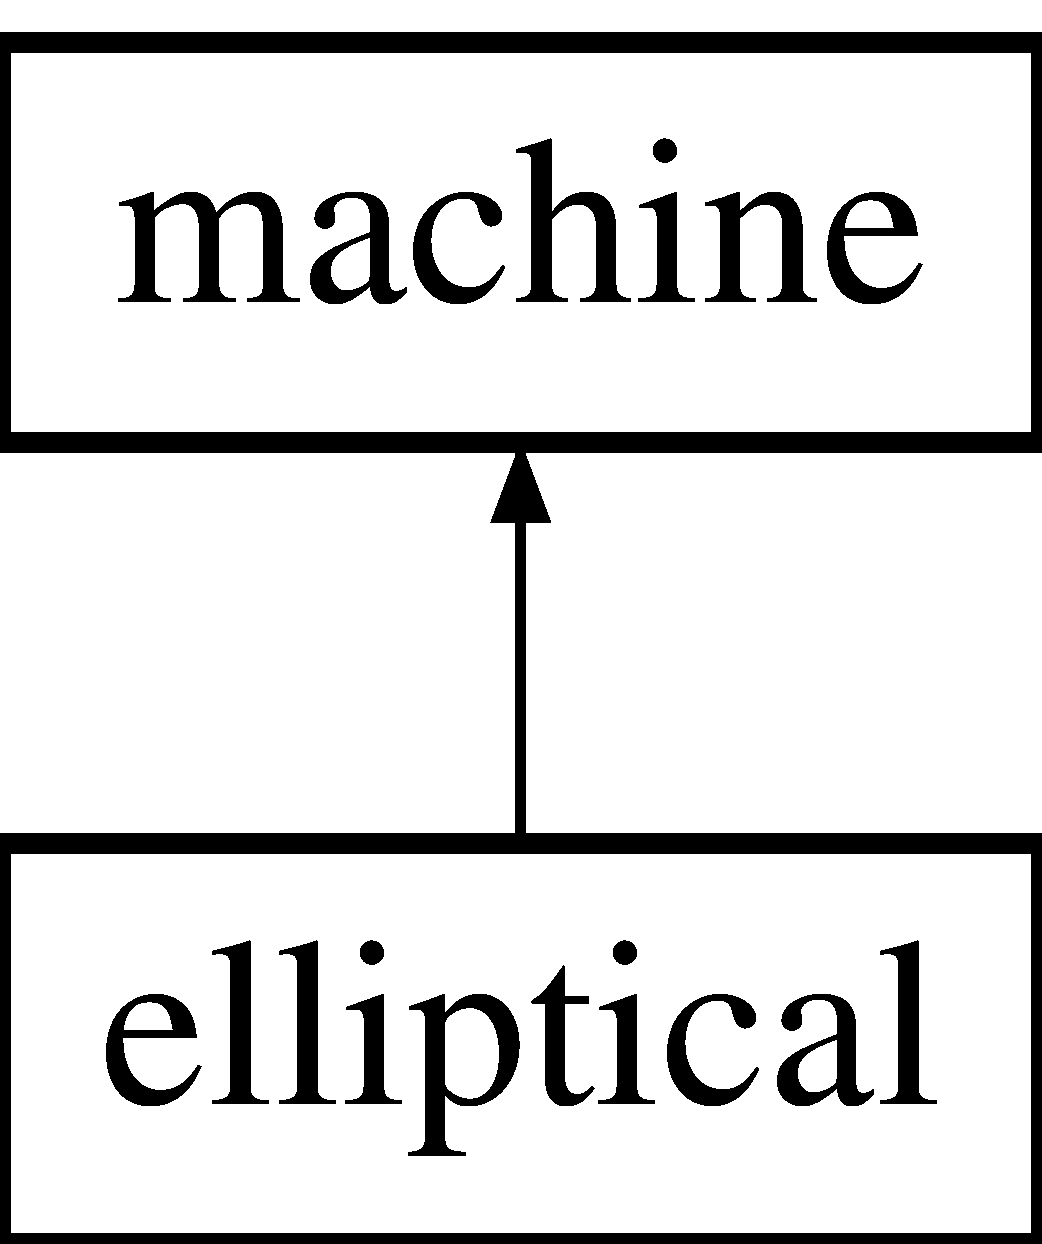
\includegraphics[height=2.000000cm]{classelliptical}
\end{center}
\end{figure}
\subsection*{Public Member Functions}
\begin{DoxyCompactItemize}
\item 
\hypertarget{classelliptical_a00cc443f8633d13f9b5a336b627d8cdf}{int {\bfseries time\-\_\-used} ()}\label{classelliptical_a00cc443f8633d13f9b5a336b627d8cdf}

\end{DoxyCompactItemize}


The documentation for this class was generated from the following files\-:\begin{DoxyCompactItemize}
\item 
elliptical.\-h\item 
elliptical.\-cpp\end{DoxyCompactItemize}

\hypertarget{classlift}{\section{lift Class Reference}
\label{classlift}\index{lift@{lift}}
}
Inheritance diagram for lift\-:\begin{figure}[H]
\begin{center}
\leavevmode
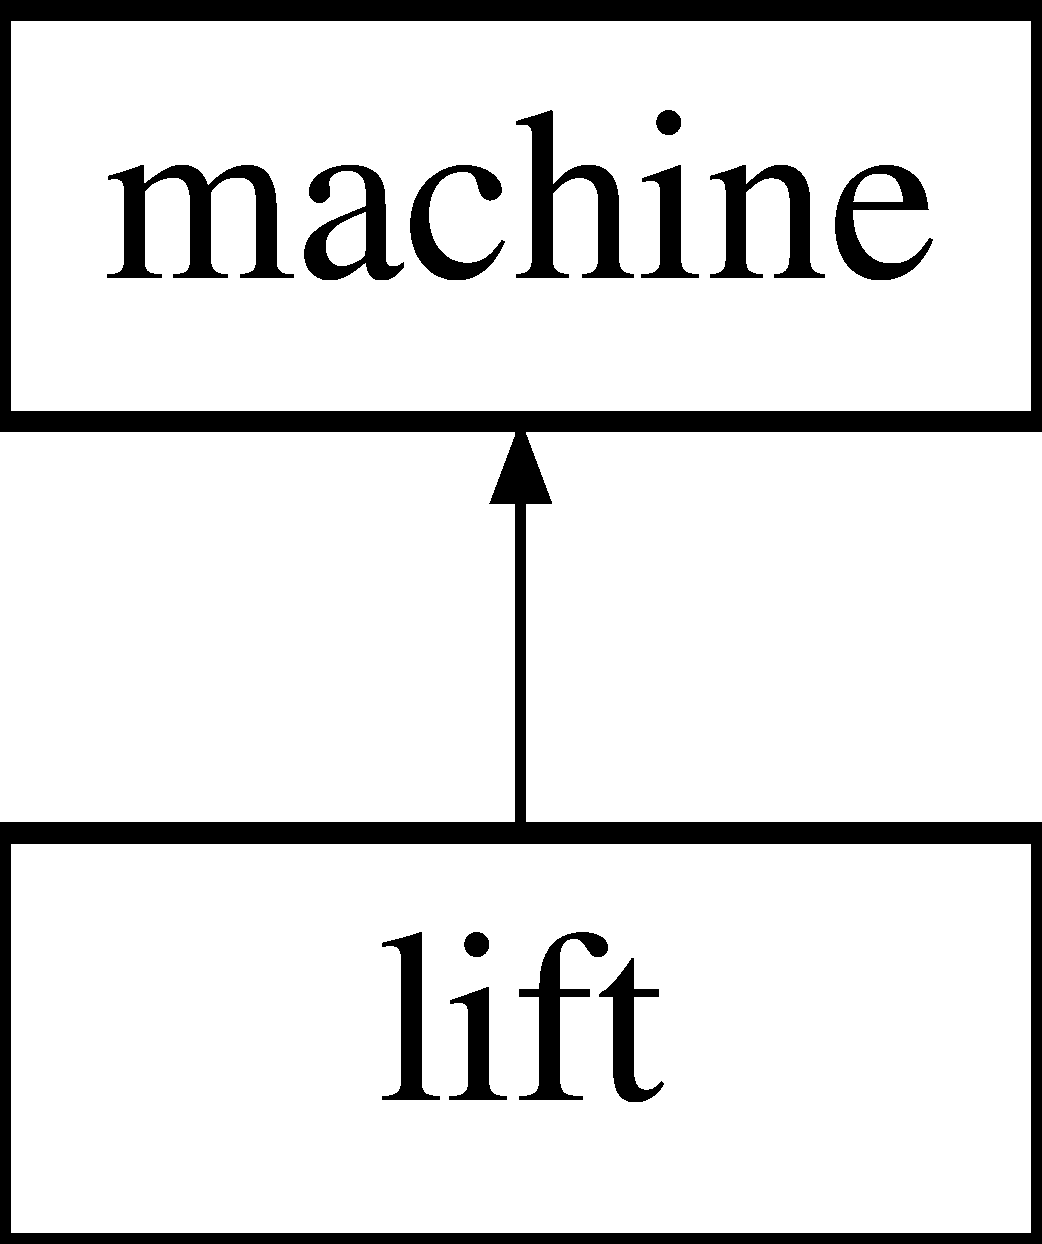
\includegraphics[height=2.000000cm]{classlift}
\end{center}
\end{figure}
\subsection*{Public Member Functions}
\begin{DoxyCompactItemize}
\item 
\hypertarget{classlift_a9f371f20603a92b21141ebc31503b0d7}{int {\bfseries repetitions} ()}\label{classlift_a9f371f20603a92b21141ebc31503b0d7}

\item 
\hypertarget{classlift_aaabecf780e0d0e1ed433fc92b301551f}{int {\bfseries weight\-\_\-lifted} ()}\label{classlift_aaabecf780e0d0e1ed433fc92b301551f}

\end{DoxyCompactItemize}


The documentation for this class was generated from the following files\-:\begin{DoxyCompactItemize}
\item 
lift.\-h\item 
lift.\-cpp\end{DoxyCompactItemize}

\hypertarget{classmachine}{\section{machine Class Reference}
\label{classmachine}\index{machine@{machine}}
}
Inheritance diagram for machine\-:\begin{figure}[H]
\begin{center}
\leavevmode
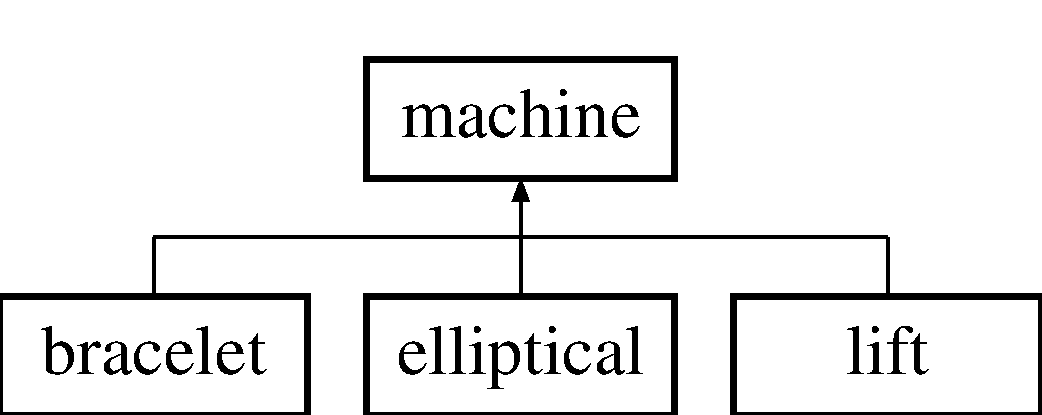
\includegraphics[height=2.000000cm]{classmachine}
\end{center}
\end{figure}
\subsection*{Public Member Functions}
\begin{DoxyCompactItemize}
\item 
\hypertarget{classmachine_a98793c9fe9044a6e6c12ded0ac96fcea}{{\bfseries machine} (std\-::string)}\label{classmachine_a98793c9fe9044a6e6c12ded0ac96fcea}

\item 
\hypertarget{classmachine_afb003d4605d7caec368eed19d73bb510}{std\-::string {\bfseries get\-\_\-name} () const }\label{classmachine_afb003d4605d7caec368eed19d73bb510}

\item 
\hypertarget{classmachine_a867d5d161df0799c6c4c3f5a39b594da}{void {\bfseries set\-\_\-name} (std\-::string)}\label{classmachine_a867d5d161df0799c6c4c3f5a39b594da}

\item 
\hypertarget{classmachine_a16f102ccb934d03c6cf8c2fd01da4b89}{\hyperlink{classmachine}{machine} $\ast$ {\bfseries clone} ()}\label{classmachine_a16f102ccb934d03c6cf8c2fd01da4b89}

\end{DoxyCompactItemize}
\subsection*{Protected Attributes}
\begin{DoxyCompactItemize}
\item 
\hypertarget{classmachine_aef2de447421299179c1417856bb3caa7}{std\-::string {\bfseries machine\-\_\-name}}\label{classmachine_aef2de447421299179c1417856bb3caa7}

\item 
\hypertarget{classmachine_ac158712554f0089431527276b170ff39}{std\-::string {\bfseries machine\-\_\-type}}\label{classmachine_ac158712554f0089431527276b170ff39}

\end{DoxyCompactItemize}


The documentation for this class was generated from the following files\-:\begin{DoxyCompactItemize}
\item 
machine.\-h\item 
machine.\-cpp\end{DoxyCompactItemize}

\hypertarget{classmember}{\section{member Class Reference}
\label{classmember}\index{member@{member}}
}
Inheritance diagram for member\-:\begin{figure}[H]
\begin{center}
\leavevmode
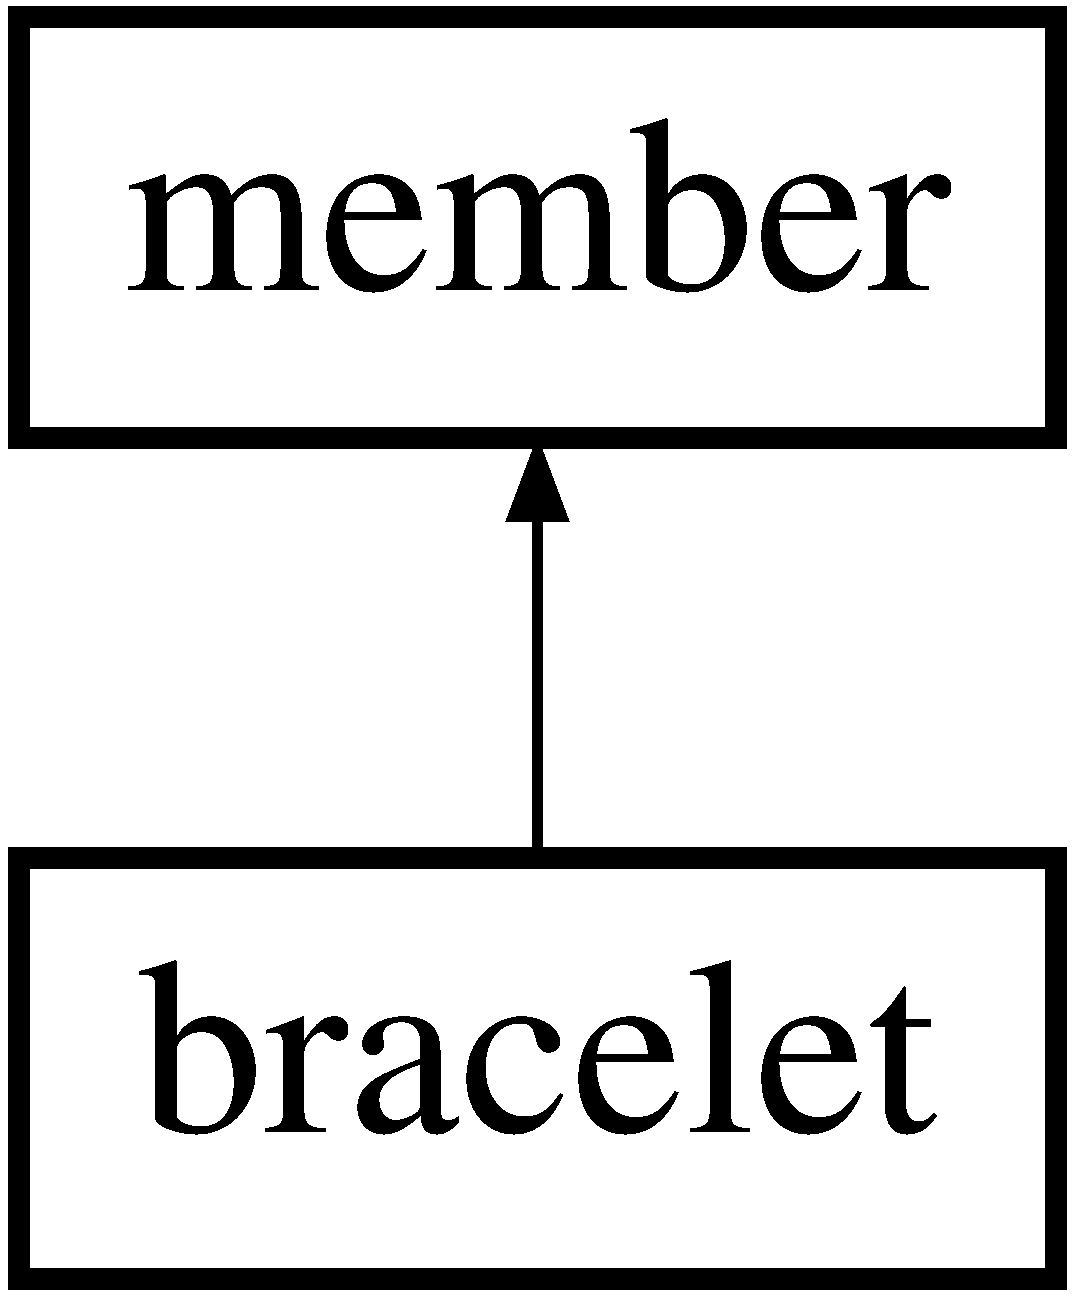
\includegraphics[height=2.000000cm]{classmember}
\end{center}
\end{figure}
\subsection*{Public Member Functions}
\begin{DoxyCompactItemize}
\item 
\hypertarget{classmember_a209a0e52f9163bfc398c5fb1dd990d61}{{\bfseries member} (char $\ast$, int)}\label{classmember_a209a0e52f9163bfc398c5fb1dd990d61}

\item 
\hypertarget{classmember_ae822170dd36d4e8733695ec2dabdeb33}{char $\ast$ {\bfseries get\-\_\-name} () const }\label{classmember_ae822170dd36d4e8733695ec2dabdeb33}

\item 
\hypertarget{classmember_a5e2b9da294c4c309d006e381ae459aa7}{int {\bfseries get\-\_\-contract} () const }\label{classmember_a5e2b9da294c4c309d006e381ae459aa7}

\item 
\hypertarget{classmember_ae9bc91157132af448c73d32fa69eaf71}{void {\bfseries set\-\_\-name} (char $\ast$)}\label{classmember_ae9bc91157132af448c73d32fa69eaf71}

\item 
\hypertarget{classmember_adf19ec5d197a949789ea2602b0e60849}{void {\bfseries renew\-\_\-contract} (int)}\label{classmember_adf19ec5d197a949789ea2602b0e60849}

\end{DoxyCompactItemize}


The documentation for this class was generated from the following files\-:\begin{DoxyCompactItemize}
\item 
member.\-h\item 
member.\-cpp\end{DoxyCompactItemize}

%--- End generated contents ---

% Index
\newpage
\phantomsection
\addcontentsline{toc}{chapter}{Index}
\printindex

\end{document}
